\begin{frame}[parent={cmap:software-testing},hasnext=true,hasprev=true]
\frametitle{Test technique}
\label{concept:test-technique}

\begin{block:concept}{Definition}
Test techniques are types of testing defined according to the
source of information used to carried out the testing activity.
\end{block:concept}

\begin{block:fact}{Test techniques and test criteria}
\begin{itemize}
    \item Each test technique has a set of associated test criteria.
\end{itemize}
\end{block:fact}
\end{frame}



\begin{frame}
\frametitle{Test technique}

\begin{block:fact}{Software test techniques}
\begin{itemize}
	\item Exhaustive testing

	\item Random testing

	\item Partition testing
	\begin{itemize}
		\item Fault-based testing

		\item Functional testing

		\item Structural testing
	\end{itemize}
\end{itemize}
\end{block:fact}
\end{frame}



\begin{frame}
\frametitle{Test technique}
\framesubtitle{Exhaustive testing}
\label{concept:exhaustive-testing}

\begin{block:concept}{Definition}
An exhaustive test executes the software with all possible value from its
input domains.
\end{block:concept}

\begin{figure}
    \centering
    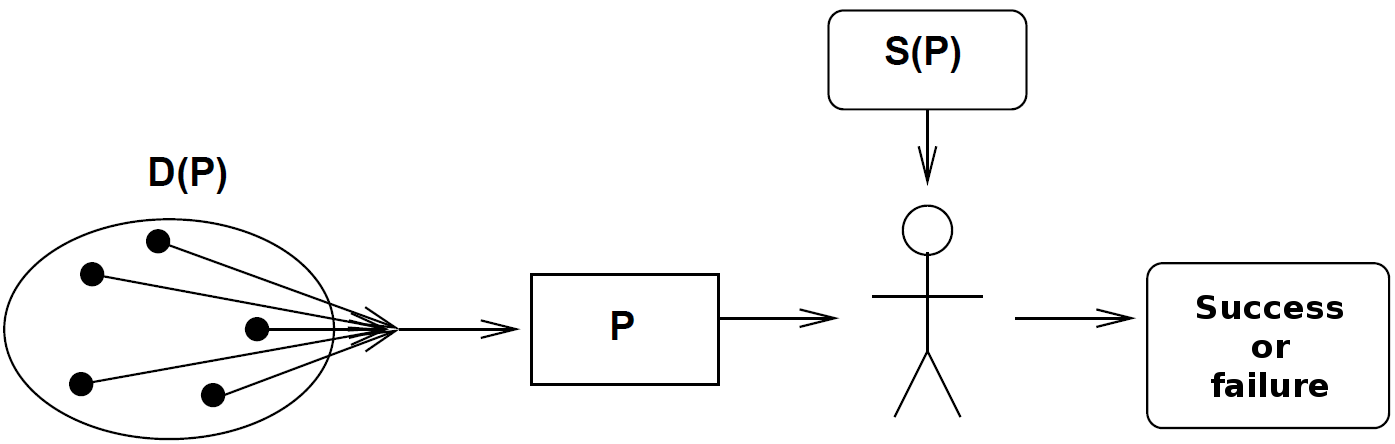
\includegraphics[width=\textwidth]{exhaustive-software-testing}
\end{figure}

\hfill
\refie{example:blech-exhaustive-testing}{\beamerbutton{Example: Exhaustive testing of the blech function}}
\end{frame}



\begin{frame}
\frametitle{Test technique}
\framesubtitle{Exhaustive testing}

\begin{block:fact}{Exhaustive testing limitations}
\begin{itemize}
	\item Can be prohibitive due to time and cost constraints for finite
	but large input domain.

	\item Impossible if the input domain is infinite.

	\item Infeasible in general.
\end{itemize}
\end{block:fact}
\end{frame}



\begin{frame}[imacidii]
\frametitle{Test technique}
\framesubtitle{Random testing}
\label{concept:random-testing}

\begin{block:concept}{Definition}
Random testing uses a systematic method to generate test cases: it
requires modeling the input space and then sampling data from the input
space randomly.
\end{block:concept}

\begin{figure}
    \centering
    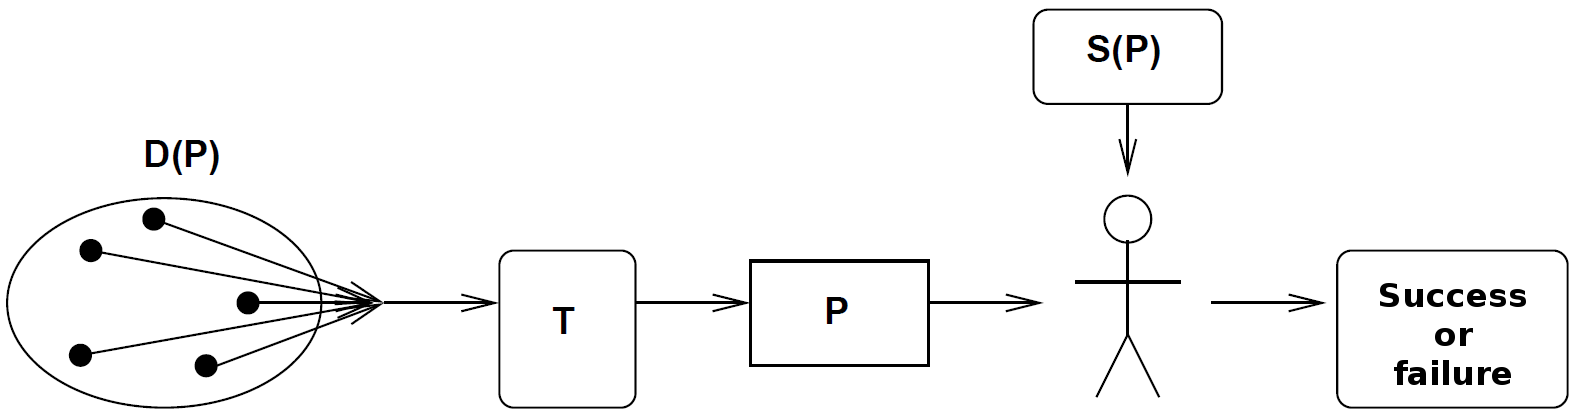
\includegraphics[width=\textwidth]{random-software-testing}
\end{figure}

\end{frame}



\begin{frame}[imacidii]
\frametitle{Test technique}
\framesubtitle{Partition testing}
\label{concept:partition-testing}

\begin{block:concept}{Definition}
Partition testing is meant any testing scheme which forces execution
of at least one test case from each subset of a partition of the input
domain
\end{block:concept}

\begin{figure}
    \centering
    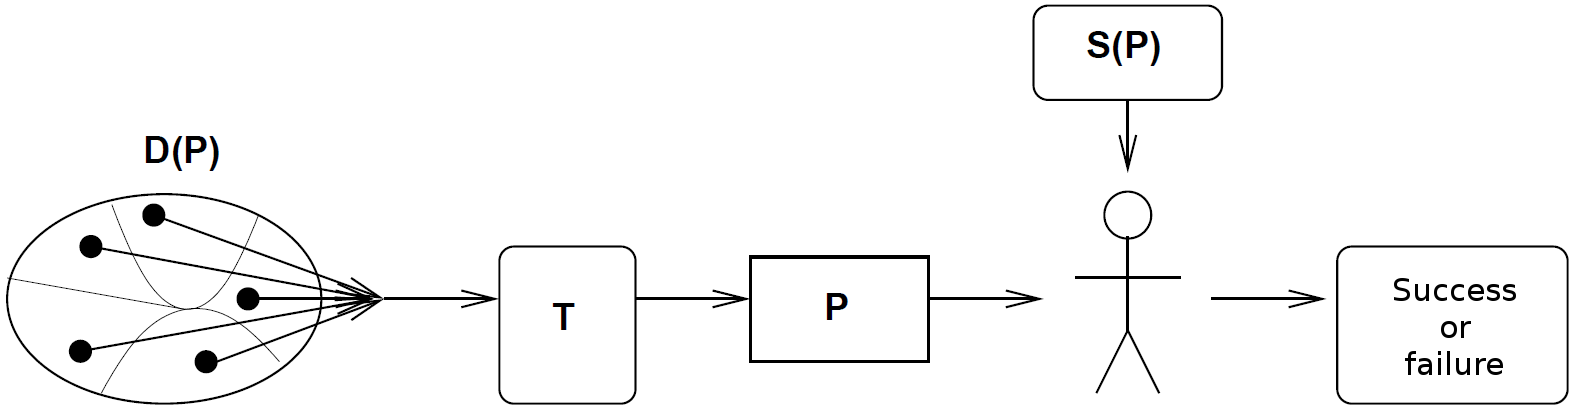
\includegraphics[width=\textwidth]{partition-software-testing}
\end{figure}
\end{frame}



\begin{frame}[imacidii]
\frametitle{Test technique}
\framesubtitle{Functional testing}
\label{concept:functional-testing}

\begin{block:concept}{Definition}
Functional testing is a technique based solely on the requirements and
specifications.
\end{block:concept}

\begin{block:fact}{}
\begin{itemize}
	\item Functional testing is also known as black box testing.

	\item Functional testing obtains test requirements from the
	software specification.
	\begin{itemize}
		\item Functional testing requires no knowledge of the internal paths,
		structure, or implementation of the software under test.
	\end{itemize}
\end{itemize}
\end{block:fact}

\hfill
\refie{example:functional-testing}{\beamerbutton{Example}}
\end{frame}



\begin{frame}[imacidii]
\frametitle{Test technique}
\framesubtitle{Structural testing}

\begin{block:concept}{Definition}
Structural testing is a technique based on the internal paths, structure,
and implementation of the software under test.
\end{block:concept}


\begin{block:fact}{}
\begin{itemize}
	\item Structural testing is also known as white box testing.

	\item Structural testing obtains test requirements from implementation
	features.
\end{itemize}
\end{block:fact}

\begin{figure}
    \centering
    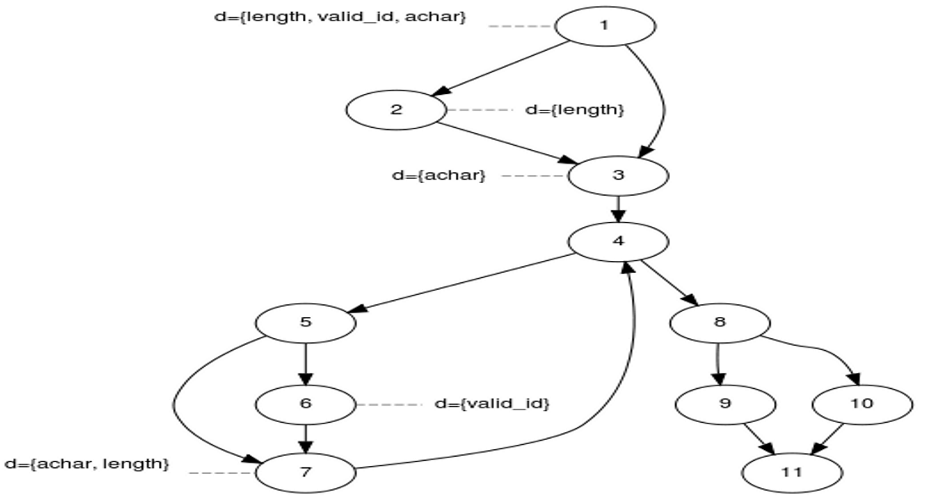
\includegraphics[width=6cm]{structural-testing}
\end{figure}
\end{frame}



\begin{frame}[imacidii]
\frametitle{Test technique}
\framesubtitle{Fault-based testing}
\label{concept:fault-based-testing}

\begin{block:concept}{Definition}
Fault-based testing is a technique in which testing is based on
historical information about common faults detected during the software
development life cycle.
\end{block:concept}

\begin{figure}
    \centering
    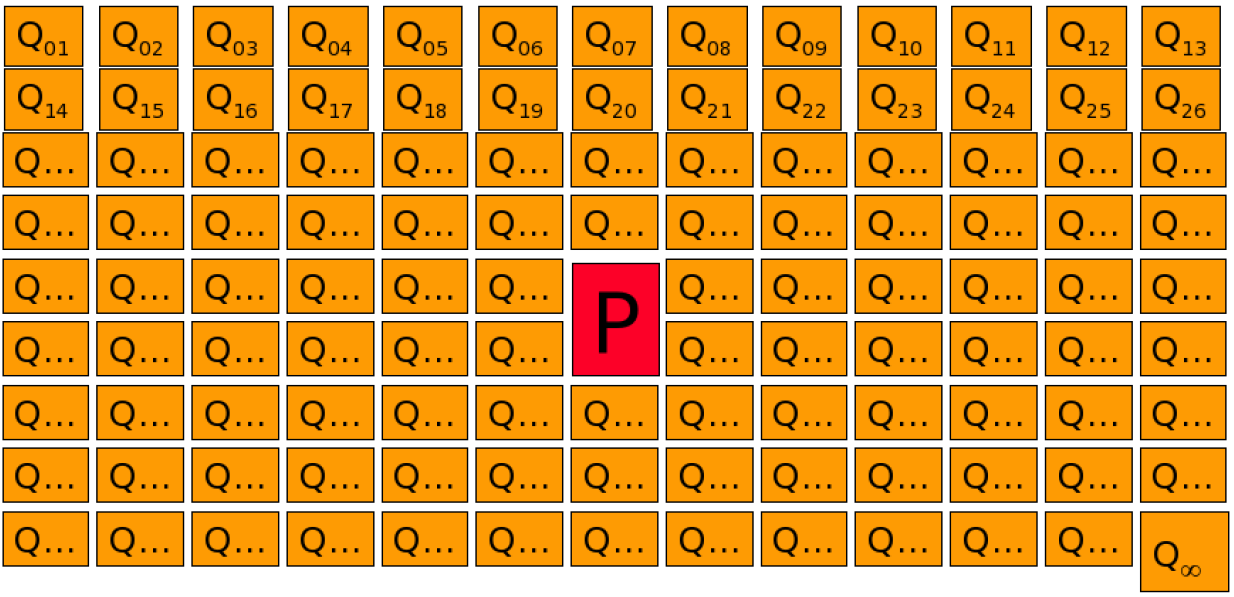
\includegraphics[width=7cm]{mutation-testing}
\end{figure}
\end{frame}
